\documentclass[a4paper,12pt]{report}
\usepackage[hidelinks]{hyperref}
\usepackage{titlesec}
\titleformat{\chapter}[display]
  {\normalfont\bfseries}{}{0pt}{\Huge}
\date{null}
\usepackage{fullpage} % changes the margin
\usepackage{setspace}
\usepackage{multirow}
\usepackage{graphicx}
\usepackage[hidelinks]{hyperref}

\title{SPM}
\author{Hetul Patel}
\date{November 2023}

\begin{document}
\begin{titlepage} % Suppresses displaying the page number on the title page and the subsequent page counts as page 1
	\newcommand{\HRule}{\rule{\linewidth}{0.5mm}} % Defines a new command for horizontal lines, change thickness here
	
	\center % Centre everything on the page
	
	%------------------------------------------------
	%	Headings
	%------------------------------------------------
	
	\textsc{\LARGE Concordia University}\\[1.5cm] % Main heading such as the name of your university/college
	

	%------------------------------------------------
	%	Title
	%------------------------------------------------
	
	\HRule\\[0.4cm]
	
	{\huge\bfseries  SOEN 6841 - Software Project Management}\\[0.4cm] % Title of your document
	
	\HRule\\[1.5cm]
	\textsc{\Large Topic Analysis and Synthesis}\\[0.5cm] % Major heading such as course name
	\textsc{\Large Leadership Is About Responsibility, Not Authority}\\[0.5cm]
	%------------------------------------------------
	%	Author(s)
	%------------------------------------------------
	
			\large
			\textit{Supervisor}\\
			Prof. Pankaj Kamthan\\[0.5cm] % Supervisor's name
% 		\end{flushright}
% 	\end{minipage}
    \vfill
    \large
			\textit{Author}\\
            Hetul Vinodbhai Patel - \textsc{40225667}\\
            
	
	\vfill\vfill\vfill\vfill% Position the date 3/4 down the remaining page
	\textbf{GitHub Address:} \url{https://github.com/Hetul79/SOEN-6841-TAS}

	%------------------------------------------------
	%	Logo
	%------------------------------------------------
	
 	\vfill\vfill
 	
\includegraphics[scale=0.5]{concordia-logo.png}\\[1cm] % Include a department/university logo - this will require the graphicx package
	 
	%----------------------------------------------------------------------------------------
	
	\vfill % Push the date up 1/4 of the remaining page
	
\end{titlepage}

%----------------------------------------------------------------------------------------

\fontsize{14}{16}\selectfont \tableofcontents
\fontsize{14}{16}\selectfont \chapter{Abstract}
\fontsize{14}{35}\selectfont This article delves into the challenges faced by leaders who find themselves in positions where their authority may be questioned, especially when they lack the experience or knowledge of their team members.Responsible leadership is based on the concept of leaders who are not isolated from the environment, who critically evaluate prevailing norms, are forward looking, share responsibility, and aim to solve problems collectively.Drawing on the principle that leadership is about responsibility, not authority, the article emphasizes the importance of leaders focusing on supporting their teams rather than dictating orders. It explores the idea that effective leadership involves a commitment to helping team members succeed, regardless of hierarchical power. The article provides insights on how leaders can navigate such situations, urging a shift from wielding authority to openly communicating responsibility for the team's success. By adopting a humble and collaborative approach, leaders can fulfill their responsibilities and become highly effective in guiding their teams to success.
\fontsize{14}{16}\selectfont \section{Key Words}
\fontsize{14}{20}\selectfont Responsibility, leadership approach, software development Cycle, authority
\fontsize{14}{16}\selectfont \chapter{Introduction}

\fontsize{14}{16}\selectfont \section{Problem Statement}
\fontsize{14}{20}\selectfont Common misconceptions perceive leadership as an authoritative role. Many leaders face challenges in gaining credibility and effectively guiding teams, particularly when holding less experience or lacking hierarchical authority.

\fontsize{14}{16}\selectfont \section{Research Questions}
\fontsize{14}{20}\selectfont 
\begin{itemize}
\item  What is the difference between authority and responsibility in terms of leadership?
\item  How to fulfill the role of leadership effectively?
\item  How does a leader's focus on responsibility over authority impact team dynamics and performance in  knowledge-intensive industries, such as software development?
\item  To what extent does a leader's emphasis on responsibility contribute to a positive work environment and employee satisfaction within a team or organization?
\item  In flat organizational structures where leaders may lack hierarchical authority, how does a leadership approach centered on responsibility influence team collaboration and productivity?
\end{itemize}

\fontsize{14}{16}\selectfont \section{Objectives}
\fontsize{14}{20}\selectfont
\begin{itemize}
\item  Investigate challenges faced by leaders in software development, particularly those with less experience.
\item  Shift the perception of leadership from authority to responsibility, promoting a more collaborative and empowering approach.
\end{itemize}

\fontsize{14}{16}\selectfont \section{Background Material}
\fontsize{14}{20}\selectfont
\begin{itemize}
\item  \textbf{Leadership in Software Development:}
In this Criteria,I have seen historical perspectives on leadership within software development teams and explore the experience from past leaders, anecdotes, or observations related to authority and disobedience. Also, it represents the evolution of leadership dynamics.
\item  \textbf{Challenges in Leading different level Experienced Teams:}
This explores the psychological aspects and challenges faced by leaders when leading teams with varying levels of experience and it has been difficult to handle leadership for those who has a little experience.Moreover, Leader should need to have knowledge of not only technical but social aspects too.So leader has to face a lot of challenges.
\item  \textbf{Evolving Leadership Paradigms:}
 This provides information about how leadership theories have evolved over time and how modern leaders are adapting to changing team structures and dynamics. It sets the stage for introducing the idea of leadership being more about responsibility than authority.
\end{itemize}

\fontsize{14}{16}\selectfont \chapter{Research Design}
\fontsize{14}{16}\selectfont \section{Responsible Leadership}
\fontsize{14}{20}\selectfont Responsible leadership is characterized as a form of leadership grounded in values, aligning performance goals with social responsibilities. It emphasizes the establishment of sustainable relationships with both internal and external stakeholders to foster mutual advantages. More precisely, responsible leaders serve as proficient individuals dedicated to achieving organizational objectives, conscientious citizens fulfilling moral obligations to society, and facilitators who prioritize the well-being of employees.
\fontsize{14}{16}\selectfont \section{Relation Between Authority and Responsibility}
\fontsize{14}{20}\selectfont  The relationship between authority and responsibility is reciprocal.In organizations with inconsistent management, the common issue of responsibility without authority hinders success. Without proper authority, tasks are neglected, and employees deviate from organizational goals. While having some authority is essential for effective delegation, an imbalance—either too little or too much authority—can lead to performance issues and misuse of delegated powers. The interconnectedness of authority and responsibility is crucial for organizational success.
\fontsize{14}{16}\selectfont \section{Leadership Challenges}
\fontsize{14}{20}\selectfont   
\begin{itemize}
\item  \textbf{Developing team:} Development of employee is main foundation of software development architecture. Leaders are facing more challenges when it is comes to development of employee and it affects a lot to organization.
\item  \textbf{Handling different perspectives:} Leaders have to handle the balancing in the team and it is extremely hard for leaders to do that as every employee has different ideas and innovation.
\item \textbf{Motivating team members:} Leaders must have better communication to keeping your employee motivated. Leaders have to understand about what employee needs so it is hard for leaders.
\item \textbf{Problem solver:} In software development, changes happen continuously so leaders need to adapt the technology in a way that it helps the organization to solve problem.
\item \textbf{Technical Knowledge:} In software development, leaders must have the knowledge of every technology so they can helps the employee. 
\end{itemize}
\fontsize{14}{16}\selectfont \section{Leadership skills for Inexperienced person}
\fontsize{14}{20}\selectfont   
\begin{itemize}
\item  \textbf{Learn from Existing Leaders:} Observe how successful leaders in your organization operate. Pay attention to their communication style, decision-making process, and how they handle conflicts.Attend leadership training programs or workshops to gain insights into various leadership styles and techniques.
\item  \textbf{Continuous Learning:} Stay updated on industry trends and best practices. This will not only enhance your technical skills but also keep you informed about the latest leadership strategies in the software engineering domain.
\item \textbf{Soft Skills Development:} Work on improving your communication skills, both written and verbal. As a leader, you'll need to effectively convey ideas and provide clear instructions.Practice active listening to understand your team members' perspectives and concerns.
\item \textbf{Seek Feedback:} Ask for feedback from colleagues and managers about your current strengths and areas for improvement.

\end{itemize}
\begin{figure}[h!]
    \centering
    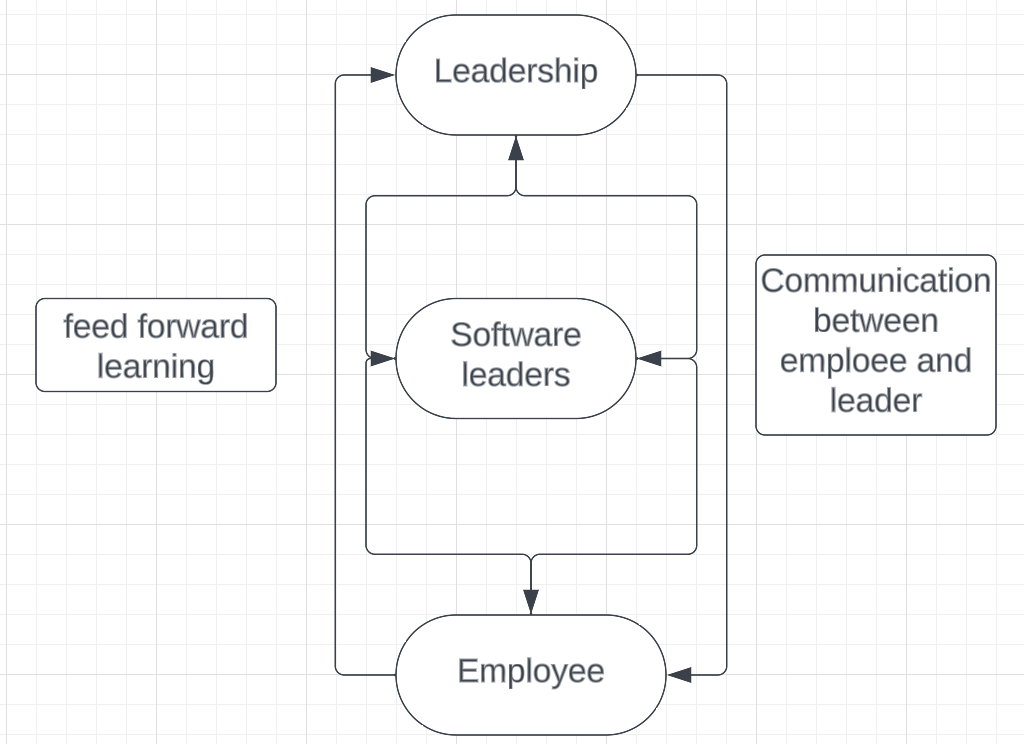
\includegraphics[scale=0.6]{Diagram.png}
    \textbf{ \caption{How responsibility and authority take place in software development}}
\end{figure}

\begin{figure}[h!]
    \centering
    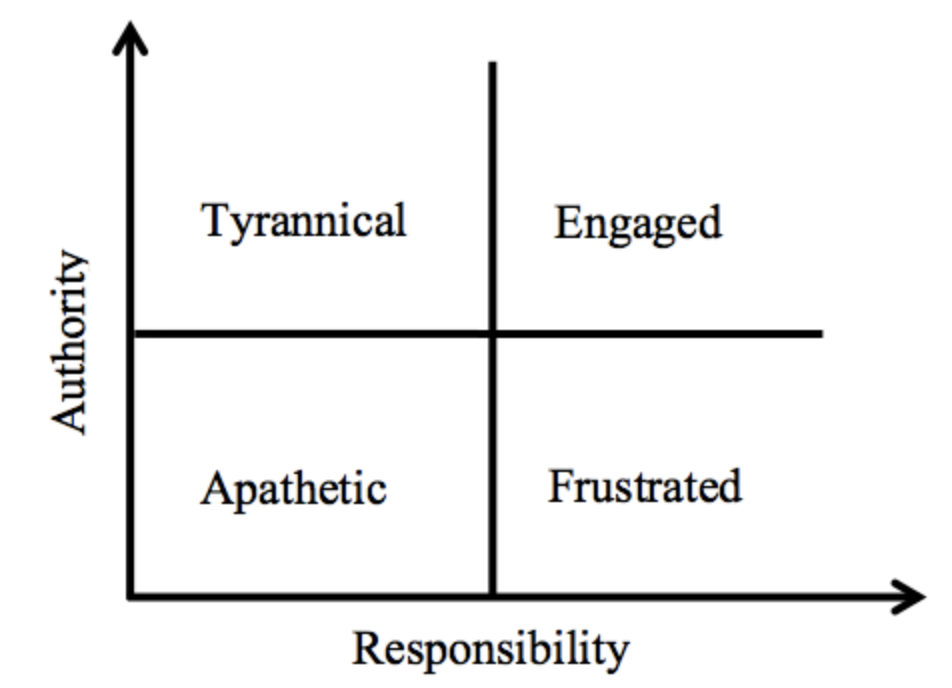
\includegraphics[scale=0.6]{diagram1.png}
    \textbf{ \caption{Connection between responsibility and authority}}
\end{figure}

\fontsize{14}{16}\selectfont \chapter{Results Obtained}
\fontsize{14}{20}\selectfont The analysis suggests that effective leadership involves a balance between responsibility and authority. While authority has its place, the emphasis on responsibility acknowledges that leadership is not merely about commanding and directing but also about fostering a sense of shared purpose and collective success within the team.

\fontsize{14}{16}\selectfont \section{Responsibility in Leadership}
\fontsize{14}{20}\selectfont   
\begin{itemize}
\item  \textbf{Long-Term Development:} Responsible leaders are focused on the long-term development and success of each team member.
\item  \textbf{Focus on Team Success:} Leaders with a focus on responsibility prioritize the success of their team members.
\item \textbf{Collaboration and Support:} Responsible leaders engage in collaborative decision-making and provide support to team members.
\end{itemize}
\fontsize{14}{16}\selectfont \section{Authority in Leadership}
\fontsize{14}{20}\selectfont   
\begin{itemize}
\item  \textbf{Hierarchy and Structure:} Authority-driven leaders often rely on hierarchical structures and clearly defined roles.
\item  \textbf{Enforcement of Rules:} Authority-focused leaders may prioritize enforcing rules and ensuring compliance.
\end{itemize}
\fontsize{14}{16}\selectfont \section{Constraint}
\fontsize{14}{20}\selectfont   
\begin{itemize}
\item \textbf{organizational and cultural restrictions:} Leaders do not able to work according to their choice because of regulation of organization. 
\end{itemize}
\fontsize{14}{16}\selectfont \chapter{conclusions}
\fontsize{14}{20}\selectfont In summary, the ability to lead effectively is a learnable skill, independent of inherent traits. Recognizing one's limitations, recruiting individuals with complementary skills, and encouraging open communication are integral to proficient leadership. Comprehending team dynamics, aligning with organizational objectives, and utilizing interpersonal strategies like attentive listening, effective communication, persuasion, and collaboration are pivotal in cultivating a devoted following. Leadership extends beyond managerial positions and is pervasive at all organizational levels. Trust and accountability, rooted in genuineness, honesty, openness, and respect, constitute essential elements for achieving success in leadership.
\fontsize{14}{16}\selectfont \section{Future Works}
\fontsize{14}{20}\selectfont  
\begin{itemize}
\item  \textbf{Suggested Improvements:} Recommends a continued emphasis on leadership as a responsibility, proposing improvements such as mentorship programs and continuous learning.
\end{itemize}

\fontsize{14}{16}\selectfont \chapter{References}
\fontsize{14}{20}\selectfont
\begin{itemize}
\item Anna Siewiorek, Eeli Saarinen, Timo Lainema , Erno Lehtinen  "Learning leadership skills in a simulated business environment" (2001)
\item Ana K. Tyssen Andreas Wald , Patrick Spieth "The challenge of transactional and transformational leadership in projects" (2008)
\item D. Visser Denise Visser Jan-Willem Mannen "Challenges in Applying Continuous Experimentation: A Practitioners' Perspective,",(2021)
\item Suzana Carmen Cismas, Ion Dona, Gabriela Ionela Andreiasu \\"Responsible Leadership" (2016)
\item Huimin Xu "The impact of heterogeneous shared leadership in scientific teams"(2023)
\item Anna Wiewiora "Adaptive network modeling of the influence of leadership and communication on learning within an organization" (2023)
\item L. Gren and P. Ralph, "What Makes Effective Leadership in Agile Software Development Teams?," (2022)
\item Trish Kerin "The importance of (process safety) leadership" (2020)
\item Mitra Madanchian a, Hamed Taherdoost "Assessment of Leadership Effectiveness Dimensions in Small and Medium Enterprises" (2019)
\item J Bus Ethics "Responsible Leadership and the Reflective CEO: Resolving Stakeholder Conflict by Imagining What Could be done"(2021)
\item Chat GPT Prompt: Used for grammar and vocabulary to make good TAS.







\end{itemize}

\end{document}